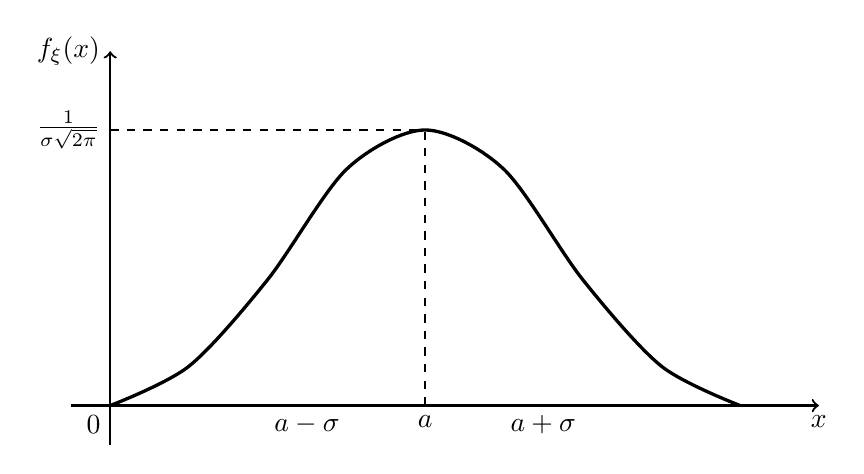
\begin{tikzpicture}
  \draw[->, thick] (-0.5, 0.5) -- (9, 0.5)
    node[pos = 1, below] {\(x\)};
  \draw[->, thick] (0, 0) -- (0, 5)
    node[pos = 1, left] {\(f_{\xi} (x)\)};

  \draw (0, 0.5) node[below left] {\(0\)};

  \draw[thick, dashed] (4, 0.5) -- (4, 4)
    node[pos = 0, below] {\(a\)};
  \draw (2.5, 0.5) node[below] {\(a - \sigma\)};
  \draw (5.5, 0.5) node[below] {\(a + \sigma\)};

  \draw[dashed, thick] (0, 4) -- (4, 4)
    node[pos = 0, left] {\(\frac{1}{\sigma \sqrt{2 \pi}}\)};

  \draw[very thick]
    plot[smooth] coordinates {
      (0, 0.5) (1, 1) (2, 2.1) (3, 3.5) (4, 4)
      (5, 3.5) (6, 2.1) (7, 1) (8, 0.5)
    };
\end{tikzpicture}